\documentclass[11pt]{article}  
\usepackage[margin=1in]{geometry}
\parindent=0in
\parskip=8pt
\usepackage{fancyhdr,amssymb,amsmath, graphicx, listings,float,subfig,enumerate,epstopdf,color,multirow,setspace,bm,textcomp}
\usepackage[usenames,dvipsnames]{xcolor}
\usepackage{hyperref}
\usepackage{graphicx}
\usepackage{tikz}
\graphicspath{{./Images}}

\pagestyle{fancy}


\begin{document} 

\lhead{Assignment \# 1}
\chead{Robert Denim Horton}
\rhead{\today}

\begin{center}\begin{Large}
CS 4720/5720 Design and Analysis of Algorithms
Homework \#1
Student: (Robert Denim Horton)
\end{Large}
\end{center}

\section*{Answers to homework problems:}

\textcolor{gray}{
% Chapter 2 : Question 1
\begin{enumerate}
	\item \quad \\
	% Question 1 : Part A
	\begin{enumerate}[(a)]
		\item  Given the formal definition of a pivotal node, a node can be difeind as such when the node of intrest exsits along every shortest possible path in a given pair of nodes.  For example, given a graph with the set of nodes $S_0$ with defined nodes $\{A, \ B, \ C, \ D, E\}$.  The graph could be represented as;\\
		\begin{center}
			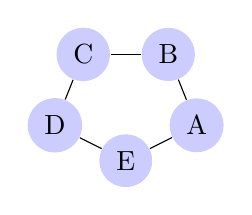
\begin{tikzpicture}[scale=0.9, auto=center, every node/.style={circle,fill=blue!20}] 
				\node(A) at (1, -0.5) {A}; 
				\node(B) at (0.6, 0.5) {B};
				\node(C) at (-0.6, 0.5) {C}; 
				\node(D) at (-1,-0.5) {D}; 
				\node(E) at (0,-1) {E}; 
				\draw(A) -- (B);
				\draw(B) -- (C);
				\draw(C) -- (D);
				\draw(D) -- (E);
				\draw(E) -- (A);
		\end{tikzpicture}
	\end{center}
As we can see in this diagram all the nodes are pivotal nodes.   Starting with node pivotal node $A$, its only pivotal node pair is $E$ and $B$, for node $B$its only pivotal node pair is $C$ and $A$, for node $C$ its only pivotal node pair is $B$ and $D$, its only pivotal node pair is $C$ and $E$, and lastly for node $E$its only pivotal node pair is $D$ and $A$.  Here we can see that every node that exsits has atleast one pair of nodes that also exists in the graph.\\
% Question 1 : Part B
	\item For a pivotal node to have two different pairs of pviotal nodes, we can again define a node with two different pairs of pivotal nodes as a node that is along the fatest path for tow nodes but with the added implication that this node is along one other pair of pivotal nodes. With the same set, $S_0$, from part a we can consruct a graph to be represnted as, 
	\begin{center}
		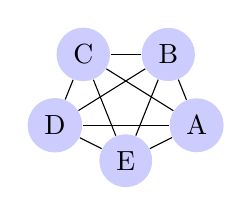
\begin{tikzpicture}[scale=0.9, auto=center, every node/.style={circle,fill=blue!20}] 
			\node(A) at (1, -0.5) {A}; 
			\node(B) at (0.6, 0.5) {B};
			\node(C) at (-0.6, 0.5) {C}; 
			\node(D) at (-1,-0.5) {D}; 
			\node(E) at (0,-1) {E}; 
			\draw(A) -- (B);
			\draw(A) -- (C);
			\draw(B) -- (C);
			\draw(B) -- (D);
			\draw(C) -- (D);
			\draw(C) -- (E);
			\draw(D) -- (E);
			\draw(D) -- (A);
			\draw(E) -- (A);
			\draw(E) -- (B);
		\end{tikzpicture}.
	\end{center}
We can see that for every node in the graph, it has atleast two different pairs of pivotal nodes.  Node $A$ has it's first pivotal nodes as $E$ and $B$ and second pair of pivotal nodes $C$ and $D$,  node $B$ has it's first set of pivotal nodes $C$ and $A$ and second pair of pivotal nodes $E$ and $D$, node $C$ has it's first set of pivotal nodes $E$ and $A$ and it's second set of pivotal nodes $B$ and $D$, node $D$ has it's first set of pivotal nodes $B$ and $A$ and second pair of pivotal nodes $C$ and $E$, node $D$ has it's first pair of pivotal nodes $B$ and $A$ and it's second set of pivotal nodes $E$ and $C$, and lastly node $E$ has it's first pair of pivotal nodes $C$ and $B$ and it's second set of pivotal nodes $A$ and $D$.\\
% Question 1 : Part C
	\item  For a graph comprised of atleast 4 nodes where a single node is pivotla for any pair of nodes that comprise a pivotal pair.  So with a different set, $S_1$, of nodes \{$A$, $B$, $C$, $D$, $X$\} we can use a graph to represnt a graph where node $X$ is the node of intrest, \\  
	\begin{center}
		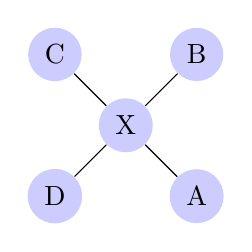
\begin{tikzpicture}[scale=0.9, auto=center, every node/.style={circle,fill=blue!20}] 
			\node(A) at (1, -1) {A}; 
			\node(B) at (1, 1) {B};
			\node(C) at (-1, 1) {C}; 
			\node(D) at (-1,-1) {D}; 
			\node(X) at (0,0) {X}; 
			\draw(A) -- (X);
			\draw(B) -- (X);
			\draw(C) -- (X);
			\draw(D) -- (X);
		\end{tikzpicture}.
	\end{center}
Here we that node $X$ has a pivotla pair with every node that is not $X$ in the graph.  So node $X$ has pivotal pairs $A$ and $C$, pivotal pair $B$ and $D$, pivotal pair $A$ and $B$, pivotal pair $C$ and $B$, pivotal pair $D$ and $A$, and pivotal pair $C$ and $D$. So six possible pairs in total.\\
	\end{enumerate}
\end{enumerate}
}
% Chapter 2 : Question 2
\textcolor{gray}{
\begin{enumerate}
\setcounter{enumi}{1}
	\item \quad \\
	\begin{enumerate}[(a)]
		\item With the formal definetion of a special type of node called a \textit{gatekeeper node}, we can identify gatekeeper node(s) as a node that must be connected by two other nodes that have no other possbile paths or connections between the two connected nodes and are limited to traversing through the gatkeeper node to get to one another  Given a set of nodes, $S_2$, comprised of nodes \{$A$, $B$, $C$, $D$, $E$, $F$\}, we can build a graph with a subset of gatekeeper nodes that comprises more than half the set of nodes in $S_1$.
	\begin{center}
		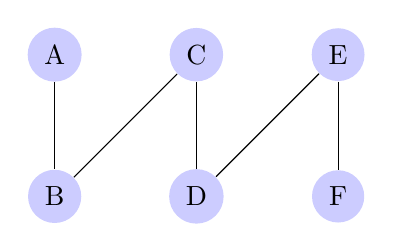
\begin{tikzpicture}[scale=0.9, auto=center, every node/.style={circle,fill=blue!20}] 
			\node(A) at (-2, 1) {A}; 
			\node(B) at (-2, -1) {B};
			\node(C) at (0, 1) {C}; 
			\node(D) at (0, -1) {D}; 
			\node(E) at (2, 1) {E};
			\node(F) at (2, -1) {F};
			\draw(A) -- (B);
			\draw(B) -- (C);
			\draw(C) -- (D);
			\draw(D) -- (E);
			\draw(E) -- (F);
		\end{tikzpicture}.
	\end{center}
As we can see, the subset of nodes \{$B$, $C$, $D$, $E$\} are all gatekeeper nodes tha must be traversed in order for specific pair of nodes to travel to one another via edges.  Further explaining we see that for the of nodes $A$ and $C$ they must travers through node $B$, qualifying node $B$ as a gatekeeper node.  The same can be said for nodes $C$, $D$, and $E$ each be a gatekeeper for their own pair of nodes that they are connected to.  $C$ is a gatekeeper for nodes $B$ and $D$, $D$ is a gatekeeper for nodes $C$ and $E$, and $E$ is a gatekeeper for nodes $D$ and $F$. 
		\item Extendeding the deffinetion of a gatekeeper there are also special kinds of gatekeeper nodes called an \textit{local gatekeeper node}.  These types typed of nodes are also connected by a pair of nodes but does not necessairly be traversed to get from one of node pairs to the other.  Given the set, $S_3$, of nodes \{$A$, $B$, $C$, $D$\} we can build a graph that consists of \textbf{only local gatekeeper nodes}.  The graph would look like;
 	\begin{center}
		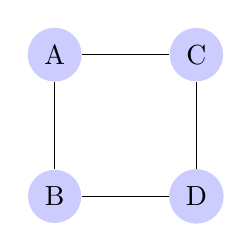
\begin{tikzpicture}[scale=0.9, auto=center, every node/.style={circle,fill=blue!20}] 
			\node(A) at (-2, 1) {A}; 
			\node(B) at (-2, -1) {B};
			\node(C) at (0, 1) {C}; 
			\node(D) at (0, -1) {D}; 
			\draw(A) -- (B);
			\draw(B) -- (D);
			\draw(D) -- (C);
			\draw(C) -- (A);
		\end{tikzpicture}.
	\end{center}
As can be seen from this graph, we notice that every pair of nodes that aren't directly connected have multiple paths or travesal to get to on another.  For example, nodes $A$ and $D$ have two paths of traversal to get to one another.  They can traverse through the first local gatekeeper, $B$, or they can traverse to each other through the second local gatekeeper $C$.  The logic can be tested on any pairs of nodes in this graph, that are not directly connected, and the conclusion will be that for every one of these pairs of nodes, there are two local gatekeeper nodes.  After stepping through the logic for every pair of nodes we will find that every node in this graph is a local gatekeeper node.
	\end{enumerate}
\end{enumerate}
}

% Chapter 2 : Question 3
\textcolor{gray}{
\begin{enumerate}
\setcounter{enumi}{2}
	\item \quad \\
	\begin{enumerate}[(a)]
		\item To first contruct such a graph lets first formally define \textit{diameter} and \textit{average distance} of a graph.  The \textbf{diameter} of a graph can be found by simply finding the longest shortest path that connects to nodes in the graph.  To find the \textbf{average distance} for a smaller and simpler looking graph, we can look through each pair of nodes that has a connection (or series of connections) and then add up all the edges that connect each combination of possible pairs of nodes.  We then divide this sum by the number of nodes that exsist on the graph.  With the provided knowledge of how to find the \textit{diameter} and \textit{average distance} we can then start to build a graph where the diameter is atleast three time larger than the average distance.\\
\quad Given a set, $S_4$, of nodes \{$A$, $B$, $C$, $D$\} we construct the first part of the graph where the nodes $A$, $B$, and $C$ are closely connected by a single node inbetween consectuvie pairs. as provided below,
   	\begin{center}
		\begin{tikzpicture}[scale=0.9, auto=center, every node/.style={circle,fill=blue!20}] 
			\node(A) at (-2, 1) {A}; 
			\node(B) at (-2, -1) {B};
			\node(C) at (0, 1) {C}; 
			\draw(A) -- (B);
			\draw(B) -- (C);
			\draw(C) -- (D);
		\end{tikzpicture}.
	\end{center}
		\item Describe how you could extend your construction to produce graphs in which the diameter exceeds the average distance by as large a factor as you’d like. (That is, for every number c, can you produce a graph in which the diameter is more than c times as large as the average distance?)\\
	\end{enumerate}
\end{enumerate}
}
\end{document}
